\input qpd-bootstrap

\begin{problem}{20260813}
  \meta{name}{Tossing the Wok}
  \meta{setter}{Sean Li}
  \meta{score}{7}
  \meta{topic}{mechanics}
  \meta{difficulty}{4}
  \meta{tags}{mechanics, rotation, energy, kinematics, rigid body}
  \meta{open}{true}
\begin{assumptions}
\item The accelerations are prescribed kinematically --- think of them as constraints imposed by the pan, not as net forces acting on a free body. Do NOT add $g$ to the net acceleration when $t < t_0$.
\end{assumptions}
\begin{center}
\begin{minipage}[c]{0.55\textwidth}
Dr.\ Wen is learning to \emph{toss the wok} --- the classical technique of jerking a pan sharply to flip its contents.

Model the pancake $\Omega$ as a uniform rigid disk of radius $R$ and planar mass density $\rho$, initially lying in the $xy$-plane with its center of mass at the origin.

At $t = 0$, two constant accelerations are applied for $[0, t_0]$:
\begin{enumerate}
    \item Angular acceleration $\alpha$ about an in-plane axis through the
    center of mass (the ``flipping axis'').
    \item Linear acceleration $\arr{a}$ of the CM, vertical component $a$.
\end{enumerate}

At $t = t_0$ the forces cease.  An \textbf{$n$-toss} is \emph{successful} if at some $t' > t_0$ the pancake returns exactly to its original spatial region, and the rigid motion between the two configurations is a pure rotation by $n\pi$ about the flipping axis.

Dr.\ Wen cooks in vacuum. Do not consider air resistance.
\end{minipage}%
\hfill
\begin{minipage}[c]{0.42\textwidth}
\centering
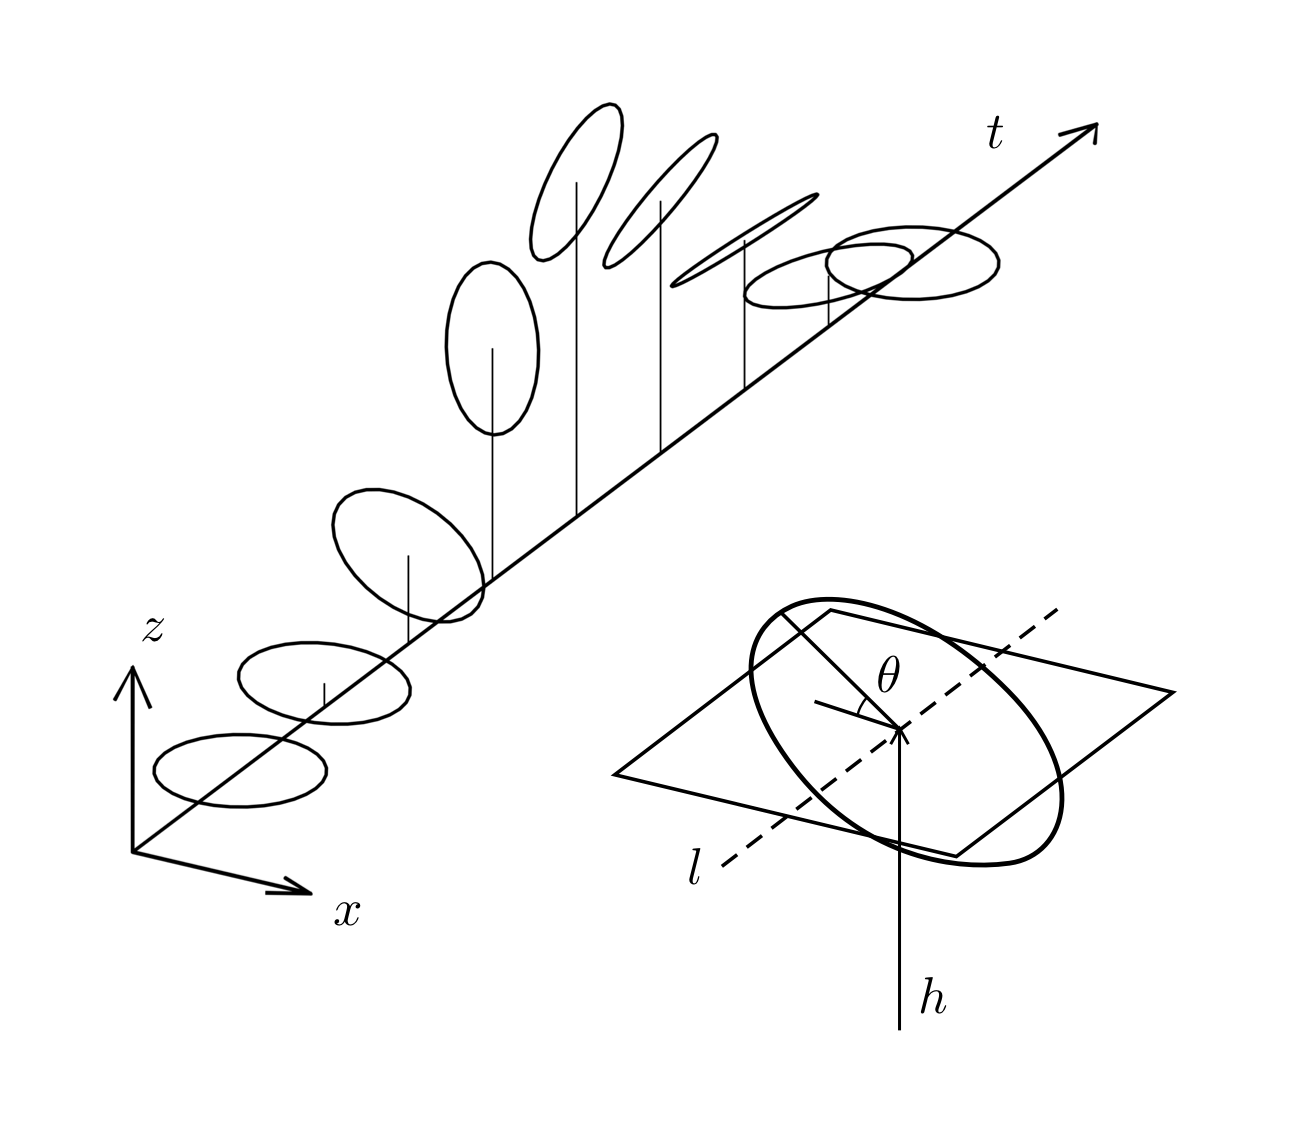
\includegraphics[width=\linewidth]{assets/20260812-1.png}
\captionof{figure}{The pancake at different $t$ during a $1$-toss.  $\theta$ is
the rotation about the flipping axis $\ell$ ($\ddot\theta=\alpha$ for $t<t_0$),
and $h$ the CM height ($\ddot h=a$ for $t<t_0$).}
\end{minipage}
\end{center}


\begin{questions}
    \item \textbf{Toss Constraint.}
    Formulate an equation that relates $n$, $\alpha$, $a$, and $t_0$ for any $n > 0$.

    \item \textbf{Toss Energy Ladder.}
    Derive the work $W$ done on the pancake as an expression containing $n$, $\alpha$, $a$ and other physical constants, and show that $W \propto n$.

    \item \textbf{Cracked Pancake.}

    \begin{center}
    \begin{minipage}[c]{0.52\textwidth}
    While tossing, Dr.\ Wen's pancake cracks exactly along the flipping axis, splitting it into two equal half-disks.  He hastily glues them back together with egg yolk, which can provide a total binding force of at most $F_y$ normal to the crack.

    During the forced phase ($t < t_0$), the rotation accelerates, creating an outward centrifugal tendency on each half-disk.  If the required centripetal force exceeds $F_y$, the halves separate and the toss is ruined. 

    Given $n$ (and the toss constraint from Q1), find the minimum $F_y$ as an expression of $n$, $a$, $\alpha$, $m$ and other physical constants needed to prevent splitting.
    \end{minipage}%
    \hfill
    \begin{minipage}[c]{0.42\textwidth}
    \centering
    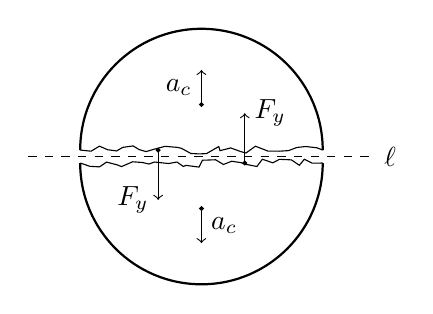
\begin{tikzpicture}[scale=1.1]
        % Upper half-disk
        \draw[thick] (-1.4,0.075) arc(180:0:1.4);
        \draw[decorate, decoration={random steps, segment length=3pt, amplitude=1.5pt}] (1.4,0.075) -- (-1.4,0.075);
        % Lower half-disk
        \draw[thick] (-1.4,-0.075) arc(180:360:1.4);
        \draw[decorate, decoration={random steps, segment length=3pt, amplitude=1.5pt}] (1.4,-0.075) -- (-1.4,-0.075);
        \draw[dashed] (-2.0,0) -- (2.0,0) node[right] {$\ell$};
        \filldraw (-0.5,0.075) circle (0.6pt);
        \draw[->] (-0.5,0.075) -- (-0.5,-0.5) node[at end,left] {$\arr{F}_y$};
        \filldraw (0.5,-0.075) circle (0.6pt);
        \draw[->] (0.5,-0.075) -- (0.5,0.5) node[at end,right] {$\arr{F}_y$};
        \filldraw (0,0.6) circle (0.6pt);
        \draw[->] (0,0.6) -- (0,1.0) node[midway,left] {$\arr{a}_c$};
        \filldraw (0,-0.6) circle (0.6pt);
        \draw[->] (0,-0.6) -- (0,-1.0) node[midway,right] {$\arr{a}_c$};
    \end{tikzpicture}
    \end{minipage}
    \end{center}
\end{questions}

\end{problem}

\begin{solution}{20260813}

Let $\mathbf q(t) = \langle h(t), \theta(t)\rangle$ with $h$ the CM vertical displacement and $\theta$ the rotation about the flipping axis.  The trajectory is piecewise-constant acceleration:
\[
\ddot{\mathbf q} =
\begin{cases}
\langle a, \alpha \rangle, & 0 \le t < t_0 \quad\text{(Forced)}\\[2pt]
\langle -g, 0 \rangle,      & t_0 \le t \le t' \quad\text{(Free fall)}
\end{cases}
\]
with $\mathbf q(0) = \dot{\mathbf q}(0) = \langle 0,0\rangle$ and $\mathbf q(t') = \langle 0, n\pi\rangle$.

\subsection*{Q1. Toss Constraint}

\textit{Phase 1} ($0 \le t < t_0$): constant acceleration, zero initial conditions.  Integrating twice:
\begin{align*}
\dot{\mathbf q}(t_0) &= t_0\langle a,\alpha\rangle,
& \mathbf q(t_0) &= \tfrac12 t_0^2\langle a,\alpha\rangle.
\end{align*}
Hence $h_0 \equiv h(t_0) = \tfrac12 a t_0^2$, $\dot h_0 \equiv \dot h(t_0) = a t_0$, $\theta_0 \equiv \theta(t_0) = \tfrac12 \alpha t_0^2$, $\dot\theta_0 \equiv \dot\theta(t_0) = \alpha t_0$.

\textit{Phase 2} ($t_0 \le t \le t'$): free motion under gravity (no torque).  Let $\Delta t = t' - t_0$.  Then
\begin{align*}
h(t') &= h_0 + \dot h_0\,\Delta t - \tfrac12 g(\Delta t)^2
      = \tfrac12 a t_0^2 + a t_0\Delta t - \tfrac12 g\Delta t^2, \\[4pt]
\theta(t') &= \theta_0 + \dot\theta_0\,\Delta t
           = \tfrac12 \alpha t_0^2 + \alpha t_0\Delta t.
\end{align*}

Success requires $h(t') = 0$ and $\theta(t') = n\pi$.  From $h(t') = 0$ (quadratic in $\Delta t$, positive root):
\[
\Delta t = \frac{t_0}{g}\Bigl(a + \sqrt{a(a+g)}\Bigr). \tag{1}
\]
From $\theta(t') = n\pi$:
\[
\Delta t = \frac{2\pi n - \alpha t_0^2}{2\alpha t_0}. \tag{2}
\]
Equating (1) and (2) gives the \textbf{toss constraint}:
\[
\boxed{\frac{\alpha t_0^2}{2g}\,\Bigl(2\sqrt{a(a+g)} + 2a + g\Bigr) = \pi n}
\qquad\text{or}\qquad
\boxed{t_0^2 = \frac{2\pi g n}{\alpha\bigl(2\sqrt{a(a+g)} + 2a + g\bigr)}}.
\]

\subsection*{Q2. Toss Energy Ladder}

The pancake is a uniform disk of radius $R$, mass $m = \pi R^2\rho$.  Its moment of inertia about the flipping axis (in-plane, through CM) is $I = \int_\Omega y^2\,\mathrm{d}m$.  In polar coordinates:
\begin{align*}
I &= \int_0^{2\pi}\!\int_0^R (r\sin\theta)^2 \rho\,r\,\mathrm{d}r\,\mathrm{d}\theta
  = \rho \int_0^{2\pi}\!\sin^2\theta\,\mathrm{d}\theta \int_0^R r^3\,\mathrm{d}r \\[4pt]
  &= \rho \cdot \pi \cdot \frac{R^4}{4}
  = \frac{1}{4} m R^2.
\end{align*}
Since the axis passes through CM, kinetic energy separates: $E(t) = m g h(t) + \tfrac12 m \dot h(t)^2 + \tfrac12 I \dot\theta(t)^2$.  At $t = 0$ all terms vanish ($E(0) = 0$).  The work done by the pan is $W = E(t_0)$:
\begin{align*}
W &= m g\!\left(\tfrac12 a t_0^2\right)
    + \tfrac12 m (a t_0)^2
    + \tfrac12\!\left(\tfrac14 m R^2\right)(\alpha t_0)^2 \\[4pt]
  &= \frac{m t_0^2}{8}\Bigl(R^2\alpha^2 + 4a^2 + 4a g\Bigr).
\end{align*}
Substituting $t_0^2$ from the toss constraint ($t_0^2 \propto n$):
\[
\boxed{W = \frac{\pi g m n}{4\alpha}\,
    \frac{R^2\alpha^2 + 4a^2 + 4a g}{2\sqrt{a(a+g)} + 2a + g}
    \;\propto\; n}.
\]

\subsection*{Q3. Cracked Pancake}

The crack splits the disk along the $x$-axis (the flipping axis) into upper ($y>0$) and lower ($y<0$) half-disks, each of mass $m/2$.

\emph{Center of mass of a uniform half-disk.}  By symmetry $\bar x = 0$.  For $\bar y$, integrate over the upper half-disk:
\[
\bar y = \frac{1}{m/2}\int_{\text{half}} y\,\mathrm{d}m
       = \frac{2}{m}\int_0^\pi\!\!\int_0^R (r\sin\theta)\,\rho\,r\,\mathrm{d}r\,\mathrm{d}\theta.
\]
With $m = \pi R^2\rho$:
\begin{align*}
\bar y &= \frac{2\rho}{\pi R^2\rho}
         \int_0^\pi \sin\theta\,\mathrm{d}\theta \int_0^R r^2\,\mathrm{d}r
       = \frac{2}{\pi R^2}\cdot \bigl[-\cos\theta\bigr]_0^\pi \cdot \frac{R^3}{3} \\[4pt]
       &= \frac{2}{\pi R^2}\cdot 2 \cdot \frac{R^3}{3}
       = \frac{4R}{3\pi}.
\end{align*}
Let $d = \bar y = 4R/(3\pi)$ be the CM distance from the flipping axis.

During the forced phase the upper half-disk's CM undergoes circular motion about the $x$-axis with $\omega(t) = \alpha t$.  The centripetal force required is
\[
F_{\text{cent}}(t) = \frac{m}{2}\,\omega(t)^2\,d
                   = \frac{2mR}{3\pi}\,\alpha^2 t^2.
\]
The egg yolk supplies this across the crack; the maximum occurs at $t = t_0$: $F_{\text{cent,max}} = \frac{2mR}{3\pi}\,\alpha^2 t_0^2$.

Using $t_0^2$ from the toss constraint (Q1):
\begin{align*}
F_{\text{cent,max}}
  &= \frac{2mR}{3\pi}\,\alpha^2\,
     \frac{2\pi g n}{\alpha\bigl(2\sqrt{a(a+g)} + 2a + g\bigr)} \\[4pt]
  &= \frac{4 R \alpha g m n}{3\bigl(2\sqrt{a(a+g)} + 2a + g\bigr)}.
\end{align*}

Therefore the egg yolk must satisfy
\[
\boxed{F_y \ge \frac{4R\alpha g m n}{3\bigl(2\sqrt{a(a+g)} + 2a + g\bigr)}}.
\]
The right-hand side is finite for any finite $\alpha$, $a$, $n$ --- a finite $F_y$ always suffices.  The required force scales linearly with both $n$ and $\alpha$: more flips or a more aggressive spin demand stronger glue.

\end{solution}

\input qpd-end